The goal of the Client Side Application (CSA) is two interact with the user.
Due to the work being developed, the CSA must:

\begin{enumerate}[noitemsep,topsep=0pt,parsep=0pt,partopsep=0pt]
  \item enable the construction of user selected requests;
  \item interact with the API to request specific resources;
  \item display the response to the user requests;
\end{enumerate}

The construction of user selected requests is done in such a way 
that it can be used to instantiate a Flying Tourist Problem,
which enables further optimization.
Following this definition, the user interface must enable the collection of:

\begin{itemize}[noitemsep,topsep=0pt,parsep=0pt,partopsep=0pt]
  \item the start city, $v_{0}$;
  \item the return city, $v_{n+1}$;
  \item a list of cities to visit $V$;
  \item the durations $D$ associated to each city in $V$;
  \item the start time/period $T_{0}$ of the trip;
\end{itemize}

Due to the computational complexity associated to this request,
the Client Side Application will not handle the optimization,
since this would consume too much of the users device resources.
Thus, upon having a complete user request, it is passed to a 
Server Side Application (SSA) to be processed.

Finally, upon receiving the response of the SSA, 
the User Interface must be updated so it can display the solutions to the request.
A solution to a request is an object which containts at least one set of flights which 
satisfies the user defined query. However, a solution to a response should 
contain several valid solutions, so the user might choose the one which is more adequate to his needs.
Furthermore, it is important that each of the flights presented contains at least the most relevant information about it.
Thus, upon presenting the solution, each flight must include, at least, the following attributes:

\begin{itemize}[noitemsep,topsep=0pt,parsep=0pt,partopsep=0pt]
  \item the flight cost;
  \item the flight duration;
  \item the date, departure and arrival time;
  \item the number of layover flights;
\end{itemize}

At this point, it is well defined what constitutes the user Input/Output,
and that the Client Side Application handles only the logic of collecting user requests,
and of preseting solutions to these requests. In its turn, the processing of the request 
is done by a third-party API - the Server Side Application.

Having a clear idea of what the CSA must do, it is possible to talk about its actual design.
The views of the User Interface can be grouped into two simple structures, the \textit{Request} view,
and the \textit{Response} view. These views enable, respectively, the construction of user requests,
and the visualization of the constructed response. There is a third view which would be very interesting to have - a \textit{Map} view.
While the Request and Response views are essential to the overall function of the application,
the Map view is not. However, a map, which could display the routes of the selected flights, aswell as other relevant information,
would certainly contribute to a better and more complete user experience.

It is also important to dicuss the design of a \textit{response} User Interface,
that is, a UI which adjust the size of the presented content according to the characteristic of the users device.
Today, the browsing of the internet occurs on a multitude of devices, which include mobile, desktop and tablet devices.
Each of these classes of products has several ranges of dimensions for the devices included in each category.
There are some mobile devices which have 3 inches screen, while others may have 6', and 
the size of the screen increases considerably as we move towards laptop and desktop screens.
Thus, upon rendering a webpage, it is important to know the size of the decive being used,
and adjust and resize the displayed content accordingly.

With this in mind, the proposed User Interface should follow the design illustrated in figure \ref{fig:UI_design}.
Notice that there are 3 views, the Response, Request, which are essential and thus are always present,
and the Map view, which is not, and thus can be discarded on some devices.


\begin{figure}[htpb]
  \centering
  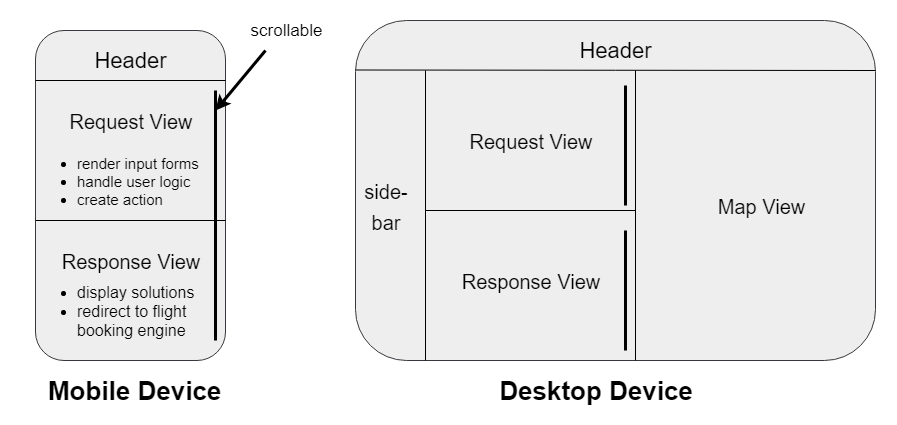
\includegraphics[width=\textwidth]{./Figures/system_design/UI_design.png}
  \caption{Proposed response User Interface for small/medium and large devices. 
  There are 2 essential views and one optional view.}
  \label{fig:UI_design}
\end{figure}




% ________________________ FRAMEWORK __________________________
%i dont think this is necessary, and i dont like its content, so dont use it.


% \vspace{5mm}
% \textbf{Framework}
% \vspace{1mm}

% The Client Side Application, or, in other words, the User Interface,
% will be designed using two javascript libraries, 
% \textit{React}, \textbf{(cite)} and \textit{Redux}, \textbf{(cite)}.
% React is a library that provides the necessary tools to build highly scalable User Interfaces.
% In its turn, Redux provides the necessary tools to organize the application logic,
% by managing the state of the application.
% React is often used together with Redux in order to build organized and modular applications. 

% The main characteristic of Redux is that it stores all the information about the application 
% in a single object, called \textit{store}. Accessing the store corresponds to accessing the state.
% This state is used by React in order to render the necessary content.
% Any user interaction that changes the state of the application, is communicated to the redux store 
% via \textit{Actions}. Actions define changes in the application. 
% In order to act upon these actions, the store uses pure functions called \textit{reducers},
% that alter the application state. 
% Using a React-Redux architecture, the state of the application is said to be \textit{the only source of truth}.
% This means that the User Interface is rendered according to the application state.
% Furthermore, React has a virtual DOM, which is used to update only the necessary parts of the UI,
% instead of reloading the entire page.
% The flow of a React Redux architecture is presented in figure \ref{fig:react_redux_cycle}

% \begin{figure}[H]
%   \centering
%   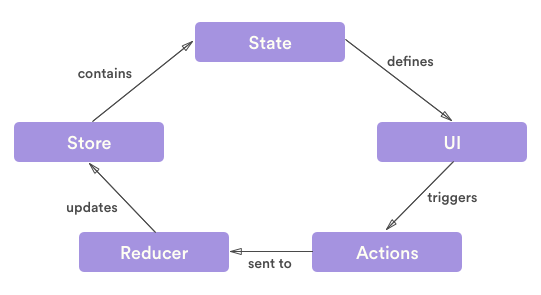
\includegraphics[width=\textwidth]{Figures/system_implementation/react_redux_flow.png}
%   \caption{The architecture of a React-Redux User Interface}
%   \label{fig:react_redux_cycle}
% \end{figure}
